\documentclass[12pt, a4paper]{article}
\usepackage{../notesheets}
%%%%%%%%%%%%%%%%%%%%%%%%%%%%%%%%%%%%%%%%%%%%%%%%%%
\author{Math 1210}
\title{Notesheet. Section 12.2: Trigonometric Functions}
\date{}

\begin{document}
\maketitle
\nameline
%%%%%%%%%%%%%%%%%%%%%%%%%%%%%%%%%%%%%%%%%%%%%%%%%%
\begin{defi}
  Given a right triangle with angle \(\theta\) marked below, we define
  our \de{trigonometric functions} as follows:\\
  \begin{minipage}{0.5\linewidth}
    \begin{itemize}
    \item \(\sin \theta =\)
    \item \(\cos \theta =\)
    \item \(\tan \theta =\)
    \item \(\csc \theta =\)
    \item \(\sec \theta =\)
    \item \(\cot \theta =\)
    \end{itemize}
    Useful mnemonic: SOHCAHTOA
  \end{minipage}
  \begin{minipage}{0.5\linewidth}
  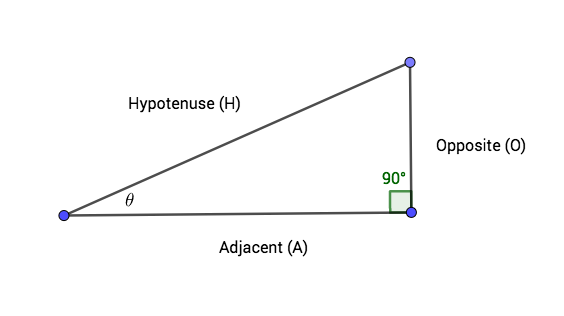
\includegraphics[scale=0.5]{images/right-triangle}    
  \end{minipage}
\end{defi}
\vspace{-0.3in}
\begin{ex}
  Consider a right triangle with \(O = 5, A = 12\). What is \(\sin
  \theta\) equal to? What is \(\cos \theta\) equal to?
\end{ex}
\vspace{-0.5in}
\begin{defi}
  The \de{unit circle} is
\end{defi}
\vspace{-1in}
\hspace{-0.25in}\begin{minipage}{0.8\linewidth}
\begin{thrm}
  Let \(P=(x,y)\) be a point on the unit circle with angle \(\theta\)
  from the \(x\)-axis. Then, \\
\end{thrm}  
\end{minipage}
\begin{minipage}{0.2\linewidth}
  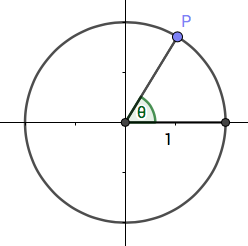
\includegraphics[scale=0.5]{images/unit-circle}
\end{minipage}
\begin{ex}
  If \(\theta = \frac{\pi}{4}\) radians, then \(P = \left(\frac{\sqrt{2}}{2},
  \frac{\sqrt{2}}{2}\right)\). If \(\theta = \frac{\pi}{6}\), then \(P =
  \left(\frac{\sqrt{3}}{2}, \frac{1}{2}\right)\).
  \begin{enumerate}
  \item Using geometry, figure out the \((x,y)\)-coordinates of \(P\)
    when \(\theta = \frac{\pi}{3}\).
  \vspace{1in}
  \item What are the \((x,y)\)-coordinates of \(P\) when \(\theta =
    -\frac{7\pi}{6}\)? What about when \(\theta = \frac{11 \pi}{4}\)?
  \vspace{1in}
  \end{enumerate}
\end{ex}
\vspace{-1.5in}
\begin{thrm}[Useful properties of sine and cosine]
  \begin{enumerate}
  \item For any value of \(\theta\), \(\sin \theta\) and \(\cos
    \theta\) are bounded by the inequalities
    \vspace{0.5in}
  \item \(\sin(\theta + 2\pi) = \) \hspace{1in} \(\cos(\theta+2\pi)=\)
  \item The graphs of \(\sin \theta\), \(\cos \theta\), and \(\tan
    \theta\) are given by
    \vspace{1.5in}
  \item \(\sin (-\theta) = \) \hspace{1in}, \(\sin \theta = 0 \iff \)
  \item \(\cos (-\theta) = \) \hspace{1in}, \(\cos \theta = 0 \iff \)
  \item \(\tan(-\theta) = \) \hspace{1in}, \(\tan \theta = 0 \iff \)
    \hspace{1in}, \(\tan(\theta + \pi) = \) 
  \end{enumerate}
\end{thrm}
\begin{ex}
  Find all values of \(\theta\) such that \(\csc \theta = -2\).
\end{ex}
%%%%%%%%%%%%%%%%%%%%%%%%%%%%%%%%%%%%%%%%%%%%%%%%%%
\end{document}
